This chapter starts the implementation of the Nuua system. Specifically, this chapter deals with the
creation of the independent logger module found in the Nuua system diagram on \autoref{fig:nuua_system}.

The logger is responsible for dealing with the error reporting of the system, so any layer can tell the logger
to store messages (a log) and at the appropriate moment a layer could make the application crash (throw an error). Those
crashes are controlled and must output a message to the user with information regarding the issue that caused the problem.

The errors that the application can throw must always include the source file, the line and the column where
the error happened. However, there might be the possibility for a crash before any source code is analyzed, meaning that a crash without
this information is still possible.

In case of an error, the reported error must be formatted accordingly and written in the standard error stream (stderr).

\section{Error design}

Error reporting plays a very important job in a compiler. Recently, GCC released a new version that improves the diagnostics
that the compiler outputs to have user-friendly errors similar to how rust does error reporting. Therefore, the error design must
be taken into consideration when designing the Nuua logger.

The \autoref{fig:nuua_errors} shows the concept for the error design.

\begin{figure}[H]
    \centering
    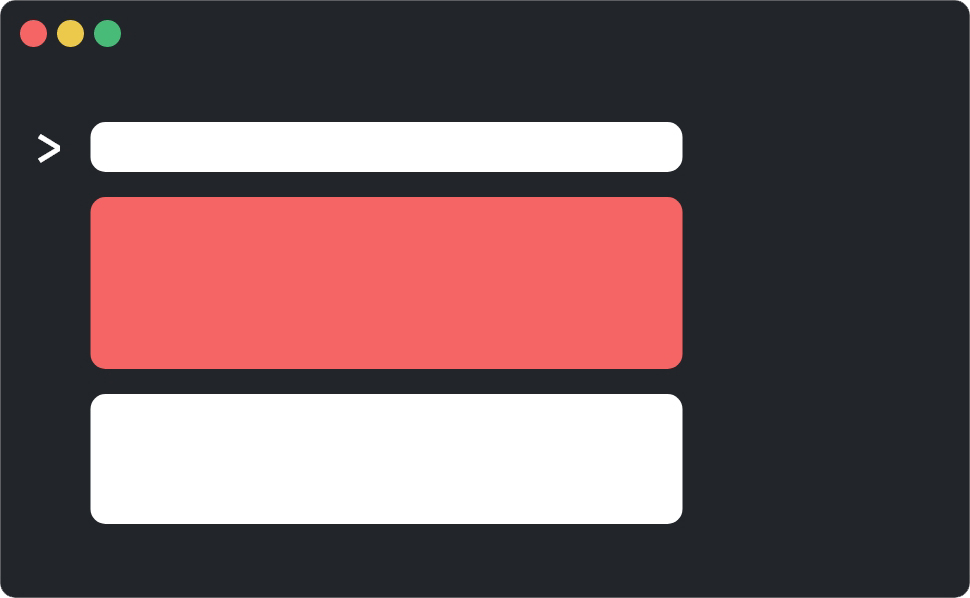
\includegraphics[width=0.4\textwidth]{errors}
    \caption{Error logging concept}
    \label{fig:nuua_errors}
\end{figure}

The first white line should include the \emph{absoltute} path of the source file followed by the line and the column where the error happened.

The red paragraph should include an error description of the error that caused the crash. This paragraph must have a fixed width to ensure
the error has a readable format.

The last white paragraph contains the line as seen in the source code of the program. The line must also include a reference to the column
where the error happened so that a quick look at the line can determine the problem.


\section{Logger entities}

The logger entity has all the properties that are mandatory fora log.
This includes the absolute file path of the source program, the line of the file where the error happened
and the column. Additionally, the error message that it has associated. A code representation is shown in
the \autoref{ls:logger_entity}.

\begin{listing}[H]
\begin{minted}{cpp}
// Represents a log entity.
class LoggerEntity {
    public:
        // Stores the file where the log comes from.
        const std::shared_ptr<const std::string> file;
        // Stores the line of the log.
        const line_t line;
        // Stores the column of the log.
        const column_t column;
        // Stores the message of the log.
        const std::string msg;
        // Creates a new log entity.
        LoggerEntity(
            const std::shared_ptr<const std::string> &file,
            const line_t line,
            const column_t column,
            const std::string &msg
        ) : file(file), line(line), column(column), msg(msg) {}
};
\end{minted}
\caption{Logger entity class}
\label{ls:logger_entity}
\end{listing}

\section{Logger class}

\autoref{ls:logger_class} shows a logger class implementation that satisfies all the previous statements.
In short, it stores a list of all the log entities and provides methods to add and remove logs. It also provides a crash
method that outputs the logs and returns an exit code without calling \texttt{exit()}.

\begin{listing}[H]
\begin{minted}{cpp}
// Represents the logger used in the whole toolchain.
class Logger
{
    // Stores all the log entities.
    std::vector<LoggerEntity> entities;
    // Displays a specific log entity.
    void display_log(const uint16_t index, const bool red) const;
    public:
        // Stores the executable path.
        std::string executable_path;
        // Adds a new entity to the entity stack.
        void add_entity(
            const std::shared_ptr<const std::string> &file,
            const line_t line,
            const column_t column,
            const std::string &msg
        );
        // Pops an entity from the entity stack.
        void pop_entity();
        // Crashes the program by displaying the entity stack
        // and further returning an apropiate exit code.
        int crash() const;
};
\end{minted}
\caption{Logger entity class}
\label{ls:logger_class}
\end{listing}

\section{Cross-platform caveat}

Due to the fact that Nuua is supported in multiple platforms, there is an important feature mentioned that must be
handled manually. The colored red output must be portable across all the major platforms. Windows is the platform that
is most special and therefore, special treatment must be taken.

For windows platforms, the C++ header \texttt{windows.h} must be included.
This header includes special functions to work with the windows terminal. The preprocessor macros
\texttt{\_WIN32} and \texttt{\_WIN64} can be used to determine if the windows header is needed.

Figure \autoref{ls:red_printf} shows the implementation of a red \texttt{printf} function working under all the major
platforms.

\begin{listing}[H]
\begin{minted}{cpp}
#if defined(_WIN32) || defined(_WIN64)
    #include <windows.h>
#endif
#include <stdio.h>
#include <stdarg.h>
#include <cstdlib>

static int red_printf(const char *format, ...)
{
    va_list arg;
    int result;
    va_start(arg, format);
    #if defined(_WIN32) || defined(_WIN64)
        HANDLE hConsole = GetStdHandle(STD_OUTPUT_HANDLE);
        CONSOLE_SCREEN_BUFFER_INFO consoleInfo;
        WORD saved_attributes;
        GetConsoleScreenBufferInfo(hConsole, &consoleInfo);
        saved_attributes = consoleInfo.wAttributes;
        SetConsoleTextAttribute(hConsole, FOREGROUND_RED);
        result = vfprintf(stderr, format, arg);
        SetConsoleTextAttribute(hConsole, saved_attributes);
    #else
        // \x1b[31m\x1b[0m = (9 + '\0')
        char *fmt = malloc(sizeof(char) * (strlen(format) + 10));
        strcpy(fmt, "\x1b[31m");
        strcat(fmt, format);
        strcat(fmt, "\x1b[0m");
        result = vfprintf(stderr, fmt, arg);
        free(fmt);
    #endif
    va_end(arg);
    return result;
}
\end{minted}
\caption{Red printf function}
\label{ls:red_printf}
\end{listing}
